% Options for packages loaded elsewhere
% Options for packages loaded elsewhere
\PassOptionsToPackage{unicode}{hyperref}
\PassOptionsToPackage{hyphens}{url}
\PassOptionsToPackage{dvipsnames,svgnames,x11names}{xcolor}
%
\documentclass[
  letterpaper,
  DIV=11,
  numbers=noendperiod]{scrreprt}
\usepackage{xcolor}
\usepackage{amsmath,amssymb}
\setcounter{secnumdepth}{5}
\usepackage{iftex}
\ifPDFTeX
  \usepackage[T1]{fontenc}
  \usepackage[utf8]{inputenc}
  \usepackage{textcomp} % provide euro and other symbols
\else % if luatex or xetex
  \usepackage{unicode-math} % this also loads fontspec
  \defaultfontfeatures{Scale=MatchLowercase}
  \defaultfontfeatures[\rmfamily]{Ligatures=TeX,Scale=1}
\fi
\usepackage{lmodern}
\ifPDFTeX\else
  % xetex/luatex font selection
\fi
% Use upquote if available, for straight quotes in verbatim environments
\IfFileExists{upquote.sty}{\usepackage{upquote}}{}
\IfFileExists{microtype.sty}{% use microtype if available
  \usepackage[]{microtype}
  \UseMicrotypeSet[protrusion]{basicmath} % disable protrusion for tt fonts
}{}
\makeatletter
\@ifundefined{KOMAClassName}{% if non-KOMA class
  \IfFileExists{parskip.sty}{%
    \usepackage{parskip}
  }{% else
    \setlength{\parindent}{0pt}
    \setlength{\parskip}{6pt plus 2pt minus 1pt}}
}{% if KOMA class
  \KOMAoptions{parskip=half}}
\makeatother
% Make \paragraph and \subparagraph free-standing
\makeatletter
\ifx\paragraph\undefined\else
  \let\oldparagraph\paragraph
  \renewcommand{\paragraph}{
    \@ifstar
      \xxxParagraphStar
      \xxxParagraphNoStar
  }
  \newcommand{\xxxParagraphStar}[1]{\oldparagraph*{#1}\mbox{}}
  \newcommand{\xxxParagraphNoStar}[1]{\oldparagraph{#1}\mbox{}}
\fi
\ifx\subparagraph\undefined\else
  \let\oldsubparagraph\subparagraph
  \renewcommand{\subparagraph}{
    \@ifstar
      \xxxSubParagraphStar
      \xxxSubParagraphNoStar
  }
  \newcommand{\xxxSubParagraphStar}[1]{\oldsubparagraph*{#1}\mbox{}}
  \newcommand{\xxxSubParagraphNoStar}[1]{\oldsubparagraph{#1}\mbox{}}
\fi
\makeatother


\usepackage{longtable,booktabs,array}
\usepackage{calc} % for calculating minipage widths
% Correct order of tables after \paragraph or \subparagraph
\usepackage{etoolbox}
\makeatletter
\patchcmd\longtable{\par}{\if@noskipsec\mbox{}\fi\par}{}{}
\makeatother
% Allow footnotes in longtable head/foot
\IfFileExists{footnotehyper.sty}{\usepackage{footnotehyper}}{\usepackage{footnote}}
\makesavenoteenv{longtable}
\usepackage{graphicx}
\makeatletter
\newsavebox\pandoc@box
\newcommand*\pandocbounded[1]{% scales image to fit in text height/width
  \sbox\pandoc@box{#1}%
  \Gscale@div\@tempa{\textheight}{\dimexpr\ht\pandoc@box+\dp\pandoc@box\relax}%
  \Gscale@div\@tempb{\linewidth}{\wd\pandoc@box}%
  \ifdim\@tempb\p@<\@tempa\p@\let\@tempa\@tempb\fi% select the smaller of both
  \ifdim\@tempa\p@<\p@\scalebox{\@tempa}{\usebox\pandoc@box}%
  \else\usebox{\pandoc@box}%
  \fi%
}
% Set default figure placement to htbp
\def\fps@figure{htbp}
\makeatother


% definitions for citeproc citations
\NewDocumentCommand\citeproctext{}{}
\NewDocumentCommand\citeproc{mm}{%
  \begingroup\def\citeproctext{#2}\cite{#1}\endgroup}
\makeatletter
 % allow citations to break across lines
 \let\@cite@ofmt\@firstofone
 % avoid brackets around text for \cite:
 \def\@biblabel#1{}
 \def\@cite#1#2{{#1\if@tempswa , #2\fi}}
\makeatother
\newlength{\cslhangindent}
\setlength{\cslhangindent}{1.5em}
\newlength{\csllabelwidth}
\setlength{\csllabelwidth}{3em}
\newenvironment{CSLReferences}[2] % #1 hanging-indent, #2 entry-spacing
 {\begin{list}{}{%
  \setlength{\itemindent}{0pt}
  \setlength{\leftmargin}{0pt}
  \setlength{\parsep}{0pt}
  % turn on hanging indent if param 1 is 1
  \ifodd #1
   \setlength{\leftmargin}{\cslhangindent}
   \setlength{\itemindent}{-1\cslhangindent}
  \fi
  % set entry spacing
  \setlength{\itemsep}{#2\baselineskip}}}
 {\end{list}}
\usepackage{calc}
\newcommand{\CSLBlock}[1]{\hfill\break\parbox[t]{\linewidth}{\strut\ignorespaces#1\strut}}
\newcommand{\CSLLeftMargin}[1]{\parbox[t]{\csllabelwidth}{\strut#1\strut}}
\newcommand{\CSLRightInline}[1]{\parbox[t]{\linewidth - \csllabelwidth}{\strut#1\strut}}
\newcommand{\CSLIndent}[1]{\hspace{\cslhangindent}#1}



\setlength{\emergencystretch}{3em} % prevent overfull lines

\providecommand{\tightlist}{%
  \setlength{\itemsep}{0pt}\setlength{\parskip}{0pt}}



 


\KOMAoption{captions}{tableheading}
\makeatletter
\@ifpackageloaded{bookmark}{}{\usepackage{bookmark}}
\makeatother
\makeatletter
\@ifpackageloaded{caption}{}{\usepackage{caption}}
\AtBeginDocument{%
\ifdefined\contentsname
  \renewcommand*\contentsname{Table of contents}
\else
  \newcommand\contentsname{Table of contents}
\fi
\ifdefined\listfigurename
  \renewcommand*\listfigurename{List of Figures}
\else
  \newcommand\listfigurename{List of Figures}
\fi
\ifdefined\listtablename
  \renewcommand*\listtablename{List of Tables}
\else
  \newcommand\listtablename{List of Tables}
\fi
\ifdefined\figurename
  \renewcommand*\figurename{Figure}
\else
  \newcommand\figurename{Figure}
\fi
\ifdefined\tablename
  \renewcommand*\tablename{Table}
\else
  \newcommand\tablename{Table}
\fi
}
\@ifpackageloaded{float}{}{\usepackage{float}}
\floatstyle{ruled}
\@ifundefined{c@chapter}{\newfloat{codelisting}{h}{lop}}{\newfloat{codelisting}{h}{lop}[chapter]}
\floatname{codelisting}{Listing}
\newcommand*\listoflistings{\listof{codelisting}{List of Listings}}
\makeatother
\makeatletter
\makeatother
\makeatletter
\@ifpackageloaded{caption}{}{\usepackage{caption}}
\@ifpackageloaded{subcaption}{}{\usepackage{subcaption}}
\makeatother
\usepackage{bookmark}
\IfFileExists{xurl.sty}{\usepackage{xurl}}{} % add URL line breaks if available
\urlstyle{same}
\hypersetup{
  pdftitle={Sustainable and Ethical Technologies for Digitally Engaged Research in the Humanities: A North-South Collaborative Lab},
  pdfauthor={HDLab CONICET},
  colorlinks=true,
  linkcolor={blue},
  filecolor={Maroon},
  citecolor={Blue},
  urlcolor={Blue},
  pdfcreator={LaTeX via pandoc}}


\title{Sustainable and Ethical Technologies for Digitally Engaged
Research in the Humanities: A North-South Collaborative Lab}
\author{HDLab CONICET}
\date{2025-08-08}
\begin{document}
\maketitle

\renewcommand*\contentsname{Table of contents}
{
\hypersetup{linkcolor=}
\setcounter{tocdepth}{2}
\tableofcontents
}

\bookmarksetup{startatroot}

\chapter*{Project/Proyecto}\label{projectproyecto}
\addcontentsline{toc}{chapter}{Project/Proyecto}

\markboth{Project/Proyecto}{Project/Proyecto}

How can a Digital Humanities (DH) project be ethical, inclusive and
(technologically and ecologically) sustainable from the start? The open
software and hardware movement has been seeking to expand global access
to digital tools by reducing cost, logistics, and knowledge barriers.
Their principles, extended beyond computing done under constraints,
could form the foundation of a global digitally-engaged humanities
commons. Likewise, the `minimal computing' movement has developed
principles to facilitate digitally engaged projects that use minimal
infrastructure to run complex humanities projects.

Could their shared principles and technologies empower students and
scholars to work more ethically and sustainably?

\begin{figure}[H]

{\centering \pandocbounded{
\includegraphics[keepaspectratio]{cover.jpg}}

}

\caption{Logo del HD LAB-CONICET}

\end{figure}%

\bookmarksetup{startatroot}

\chapter{Sobre minimal computing}\label{sobre-minimal-computing}

\section{Definición inicial y
orígenes}\label{definiciuxf3n-inicial-y-oruxedgenes}

Las primeras definiciones de \emph{minimal computing} fueron formuladas
en el marco del grupo \href{http://www.globaloutlookdh.org/}{Global
Outlook::Digital Humanities (GO::DH)} hacia 2014--2015, en los debates
coordinados por Alex Gil y Jentery Sayers. El grupo GO::DH, fundado en
2012, se propuso abrir espacios de intercambio entre investigadores de
contextos geográficos y lingüísticos marginados en la conversación
dominante de las Humanidades Digitales. En este marco, la \emph{minimal
computing} fue presentada como un modo de contrarrestar desigualdades
estructurales: se trata de diseñar y mantener proyectos que puedan
operar en condiciones de baja conectividad, con hardware limitado o con
escasos recursos económicos, asegurando así que la investigación digital
no dependa exclusivamente de entornos privilegiados de infraestructura.

En el \href{https://go-dh.github.io/mincomp/about/}{sitio del proyecto}
se define a la \emph{minimal computing} como: ``computing done under
some set of significant constraints of hardware, software, education,
network capacity, power, or other factors'' (computación realizada bajo
un conjunto de restricciones significativas de hardware, software,
formación, capacidad de red, energía u otros factores). A esta
definición inicial Alex Gil (2015) añade que la \emph{minimal computing}
``It is also the computing we choose to do for the sake of ethics,
sustainability, and access'' (también es el tipo de computación que uno
decide realizar de manera consciente, para reducir la dependencia
tecnológica y fomentar la sostenibilidad y la accesibilidad).

Las primeras ediciones digitales que se realizaron siguiendo estos
principios buscaban una simplicidad absoluta, en la que se prioriza la
preservación y transmisión del texto, y que en su mayoría se
desarrollaron utilizando Markdown como lenguaje de marcado, lo que
implica requisitos mínimos, no sólo en términos de infraestructura, sino
también de la curva de aprendizaje requerida para su uso.

Algunos ejemplos de ediciones digitales realizadas con estos criterios
son el sitio sobre \emph{minimal computing} de GO::DH y la revista
\emph{archipelagos}:

\href{https://go-dh.github.io/mincomp/}{\pandocbounded{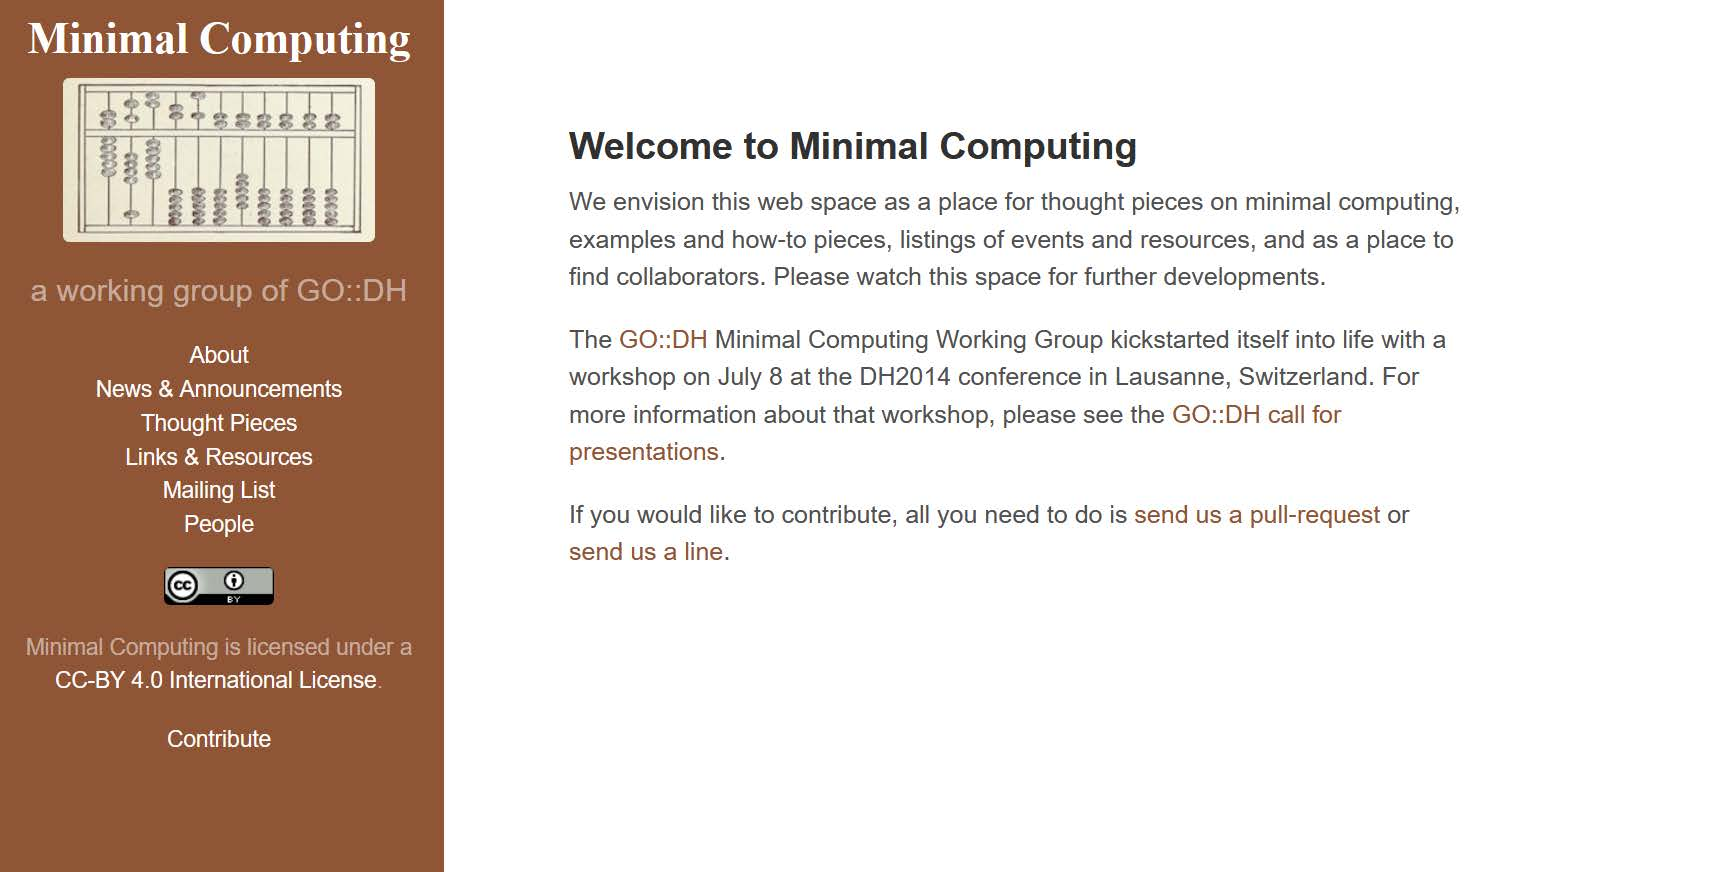
\includegraphics[keepaspectratio]{assets/mc-image1.jpg}}}

El sitio \href{https://go-dh.github.io/mincomp/}{Minimal Computing} es
el espacio oficial del grupo de trabajo homónimo dentro de GO::DH.
Funciona como un punto de encuentro para publicar ensayos, tutoriales,
recursos, noticias y convocatorias sobre el enfoque minimalista en
humanidades digitales.

\href{https://archipelagosjournal.org/index.html}{\pandocbounded{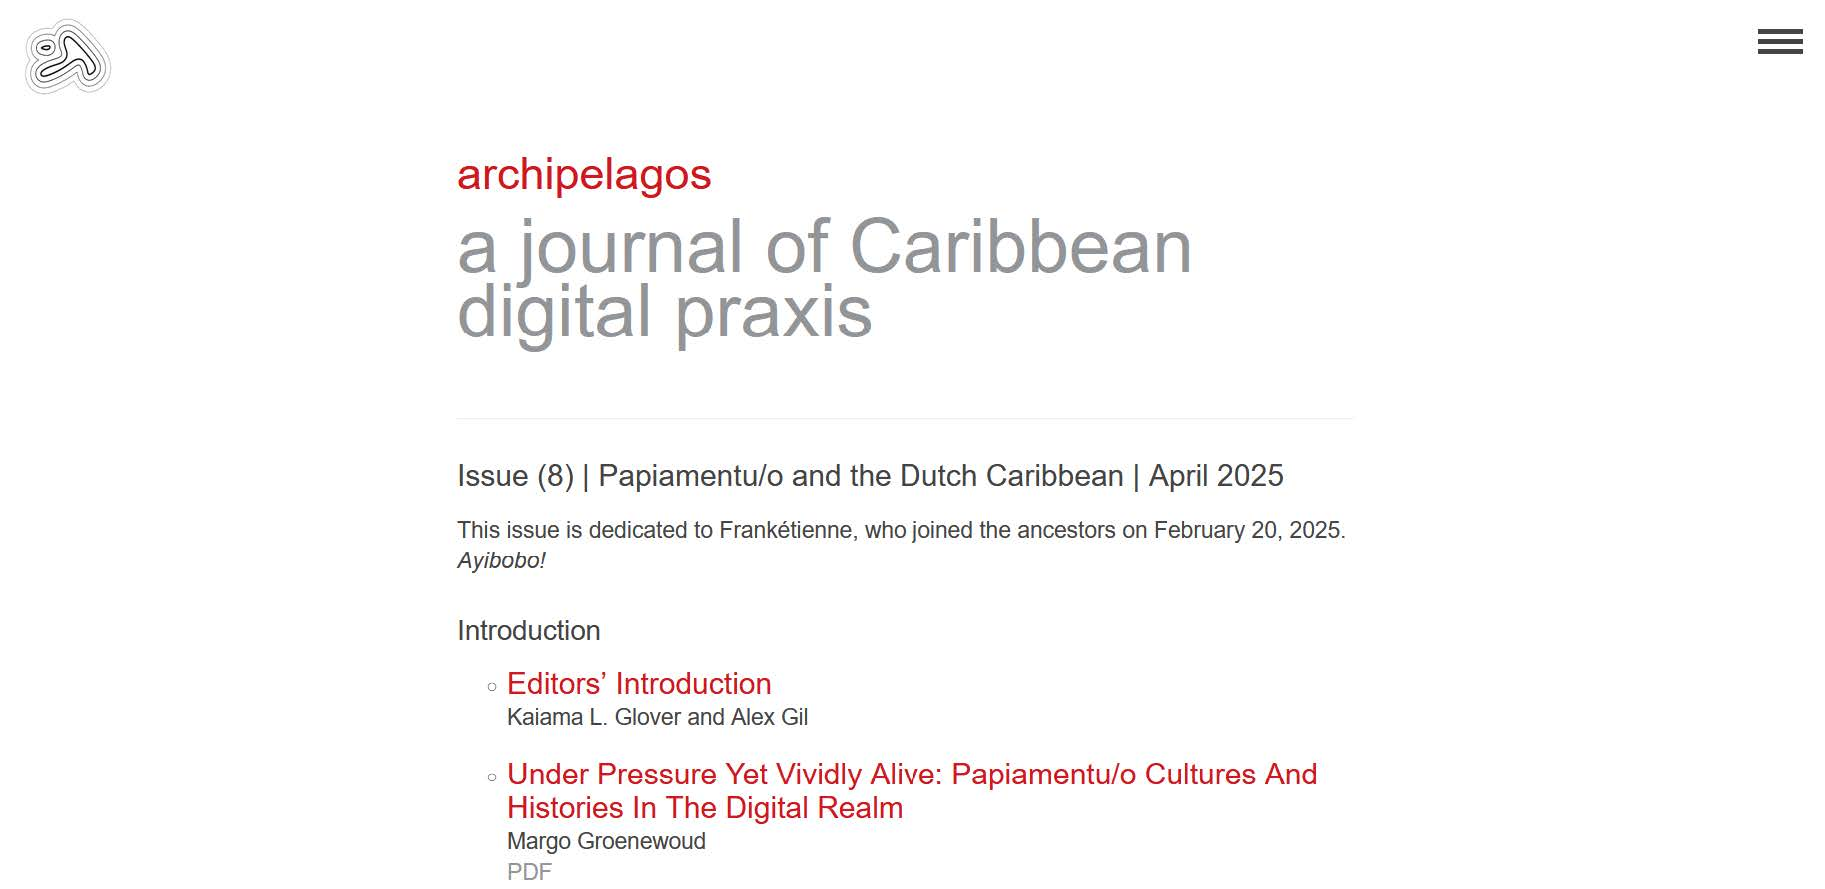
\includegraphics[keepaspectratio]{assets/mc-image2.jpg}}}

La revista
\href{https://archipelagosjournal.org/index.html}{\emph{archipelagos: a
journal of Caribbean digital praxis}} es una publicación académica de
acceso abierto dedicada a las prácticas digitales en el Caribe y sus
diásporas. Utiliza herramientas de código abierto y una infraestructura
ligera de sitios estáticos que facilita su sostenibilidad, reduce costos
y garantiza accesibilidad incluso en contextos de baja conectividad.

\section{\texorpdfstring{Ediciones digitales con \emph{minimal
computing} en el contexto
hispanohablante}{Ediciones digitales con minimal computing en el contexto hispanohablante}}\label{ediciones-digitales-con-minimal-computing-en-el-contexto-hispanohablante}

Si bien los primeros ejemplos de ediciones digitales realizadas con
minimal computing optaron en su mayoría por Markdown como lenguaje de
marcado a causa de su mayor simplicidad, desde temprano surgieron
propuestas que buscaron incorporar la codificación de texto en XML-TEI,
el estándar más utilizado para la Edición Filológica Digital y otras
disciplinas de las Humanidad y las Ciencias Sociales, al proceso de
publicación en sitios estáticos. En el contexto hispanohablante, un
ejemplo temprano de esta tendencia es el
\href{https://minilazarillo.github.io/index.html}{\emph{mini
lazarillo}}, una edición digital mínima del \emph{Lazarillo de Tormes}
(1554), creada por estudiantes del Departamento de Culturas
Latinoamericanas e Ibéricas de la Universidad de Columbia. Ofrece una
edición de lectura sencilla, una edición anotada y una versión
facsimilar.

\href{https://minilazarillo.github.io/index.html}{\pandocbounded{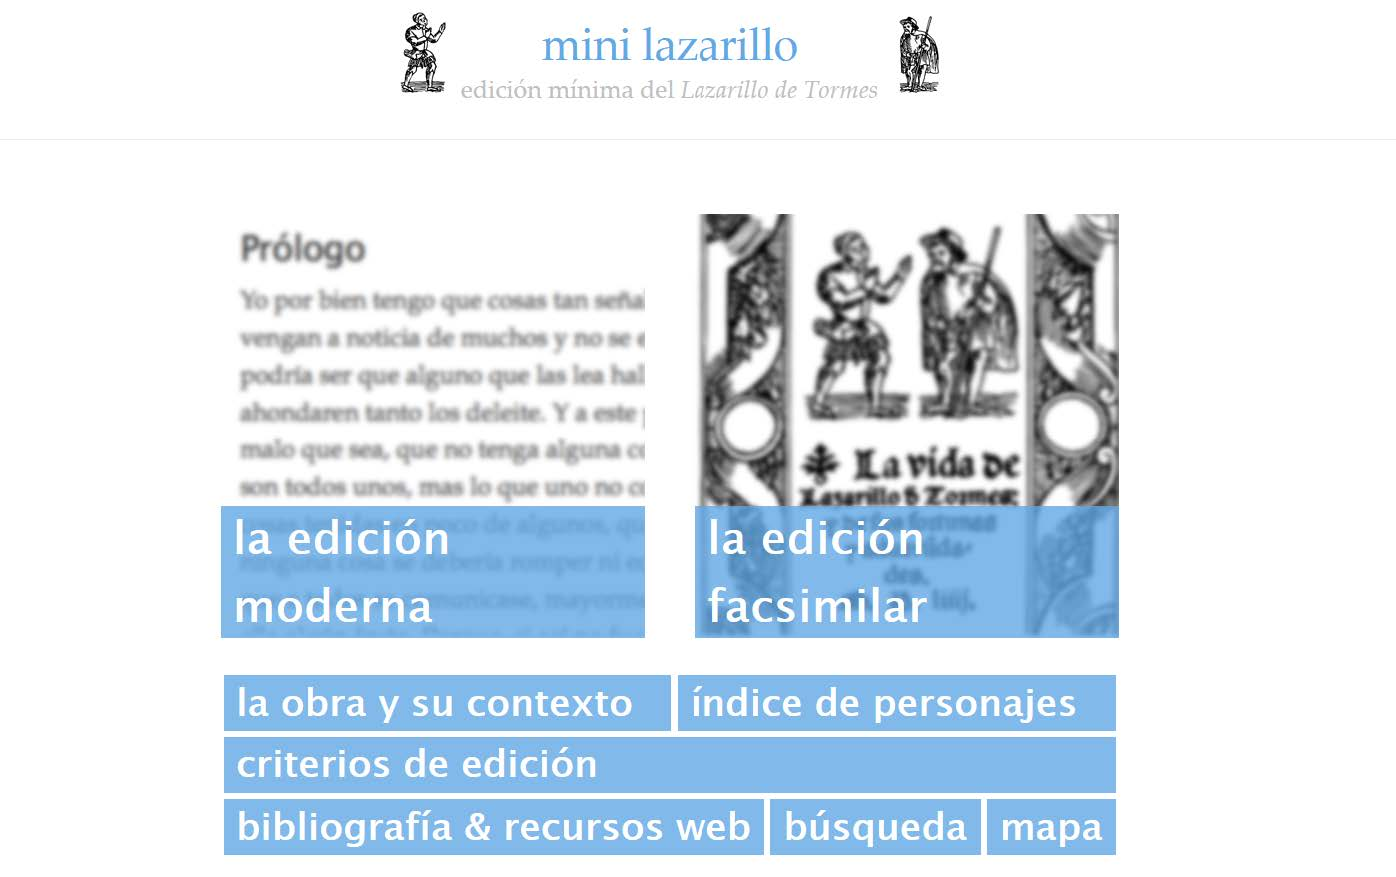
\includegraphics[keepaspectratio]{assets/mc-image3.jpg}}}

En los últimos años, la \emph{minimal computing} se ha consolidado como
un paradigma crítico que intenta dar respuesta a las crecientes demandas
técnicas, económicas y ecológicas de la investigación digital. Rio
Riande (2022b, pp.~8-9) la define como ``un conjunto de principios y
tecnologías de código abierto que permiten capacitar a los estudiantes e
investigadores para trabajar de manera autónoma y tener más control
sobre el futuro de sus propios proyectos''. Esta propuesta dialoga con
las reflexiones de Alex Gil, quien ya en 2015 planteaba que la elección
de tecnologías debía guiarse por la pregunta ``what do we need?''. Años
más tarde, junto con Risam, complejizó este marco con una serie de
interrogantes que incorporan tanto los recursos disponibles como las
prioridades y concesiones que implica cada proyecto: ``1) what do we
need?; 2) what do we have?; 3) what must we prioritize?; and 4) what are
we willing to give up?'' (Risam y Gil, 2022). Estas preguntas evidencian
que la \emph{minimal computing} funciona no sólo como un conjunto de
soluciones técnicas, sino también como una metodología crítica y
reflexiva sobre los límites y posibilidades de la creación digital.

En este contexto, la propuesta de la \emph{minimal computing} no
consiste en reducir la complejidad de las prácticas académicas, sino en
priorizar la eficiencia, la sostenibilidad y la autonomía en el diseño
de proyectos. Frente a las ediciones digitales alojadas en sitios
dinámicos que requieren infraestructuras costosas y una constante
inversión de recursos, esta aproximación enfatiza el uso de sitios
estáticos y herramientas de código abierto, como Jekyll y Github, que
permiten construir entornos de publicación sostenibles, de bajo consumo
energético y más fáciles de mantener (Rio Riande, 2022a; Viglianti et
al., 2022). En este sentido, la \emph{minimal computing} no significa
renunciar a la complejidad filológica, sino repensarla desde una ética
del diseño orientada a la accesibilidad y a la equidad en la circulación
del conocimiento.

Este enfoque adopta los principios de la \emph{minimal computing} en
cuanto a la independencia de infraestructuras costosas y poco
sustentables, pero busca aprovechar al máximo el potencial del uso de
sitios estáticos y herramientas de código abierto para crear objetos
digitales complejos, con diferentes formas de visualización y
acompañamiento en la lectura del texto, aunque esto signifique tener que
abordar una curva de aprendizaje más elevada.

Un ejemplo de esta tendencia puede encontrarse en la edición digital
enriquecida del
\href{https://hdlab.space/viaje-al-rio-de-la-plata/}{Viaje al Río de la
Plata (1534--1554) de Ulrich Schmidel}, elaborada por el
\href{https://hdlab.space/}{HDLab-CONICET}, que acompaña la edición del
texto con recursos como un mapa interactivo del itinerario desde Amberes
hacia Suramérica, anotaciones, visualizaciones, notebooks y un
vocabulario controlado:

\href{https://hdlab.space/viaje-al-rio-de-la-plata/}{\pandocbounded{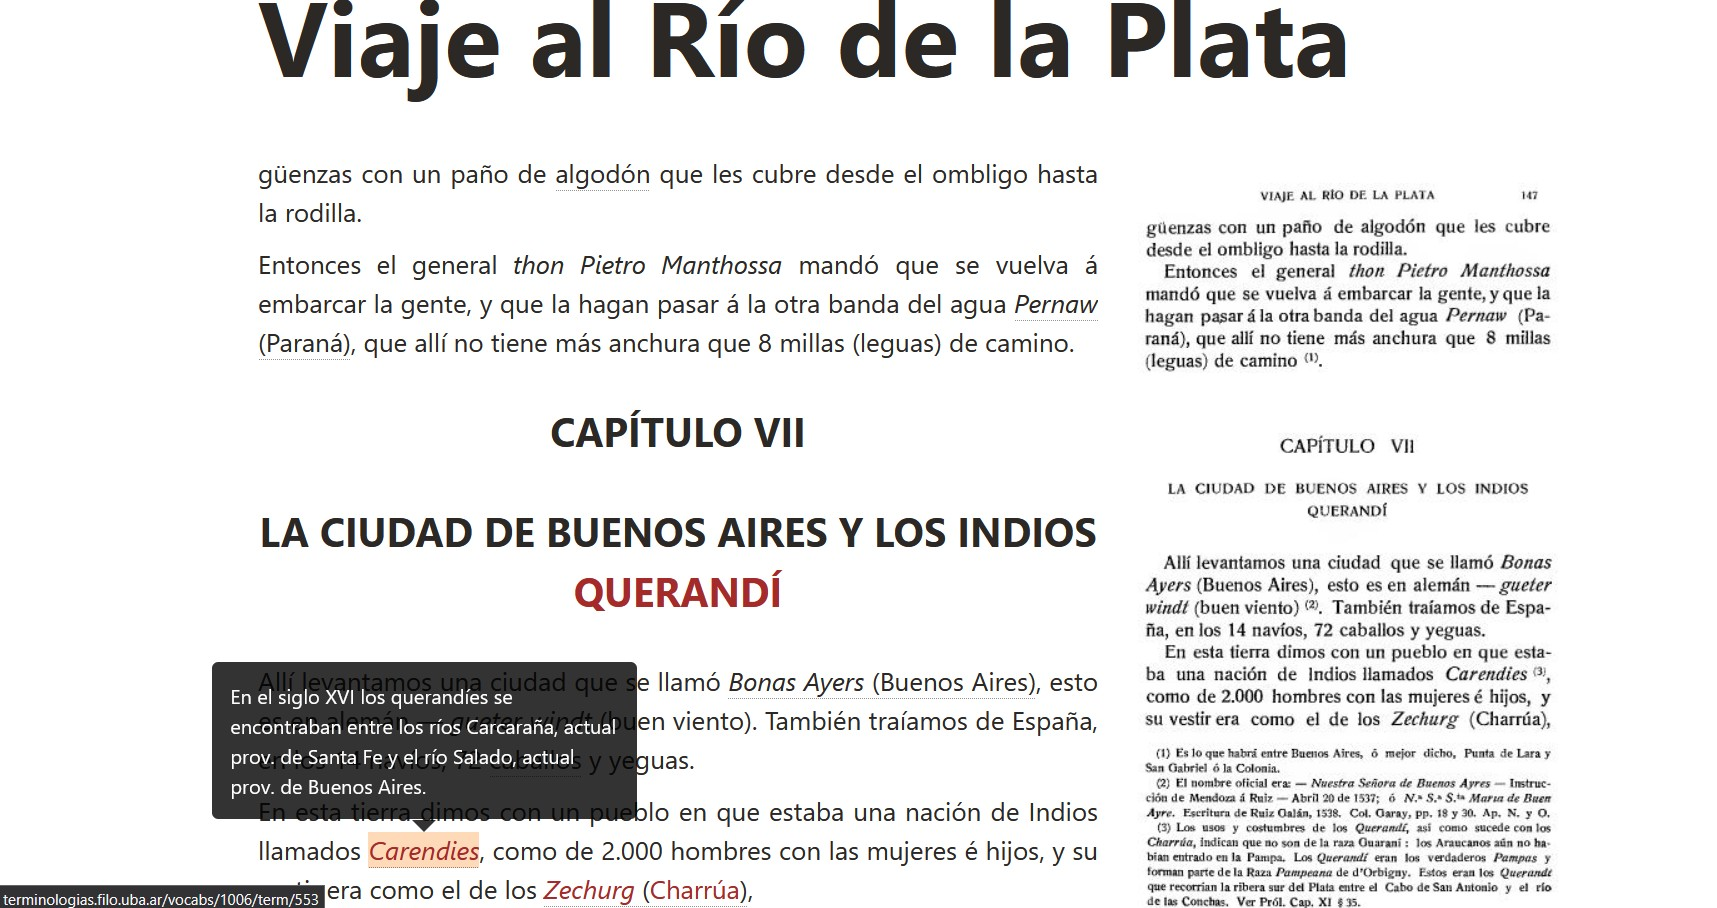
\includegraphics[keepaspectratio]{assets/mc-image4.jpg}}}

\section{\texorpdfstring{Colecciones con \emph{minimal
computing}}{Colecciones con minimal computing}}\label{colecciones-con-minimal-computing}

En los últimos años también fue cobrando relevancia el uso de sitios
estáticos para la creación de colecciones digitales. A diferencia de las
bases de datos dinámicas, las colecciones generadas con herramientas
como Jekyll, Hugo o Wax ofrecen ventajas de sostenibilidad, bajo consumo
de recursos y facilidad de preservación a largo plazo, garantizando
además independencia respecto de plataformas propietarias. Si bien

sostenibilidad y accesibilidad en proyectos que trabajan con patrimonio
cultural, como el archivo crítico digital de \emph{La dama boba} y la
colección de ediciones diplomáticas de la Colección Foulché-Delbosc:

\href{https://celioht.github.io/damaboba/}{\pandocbounded{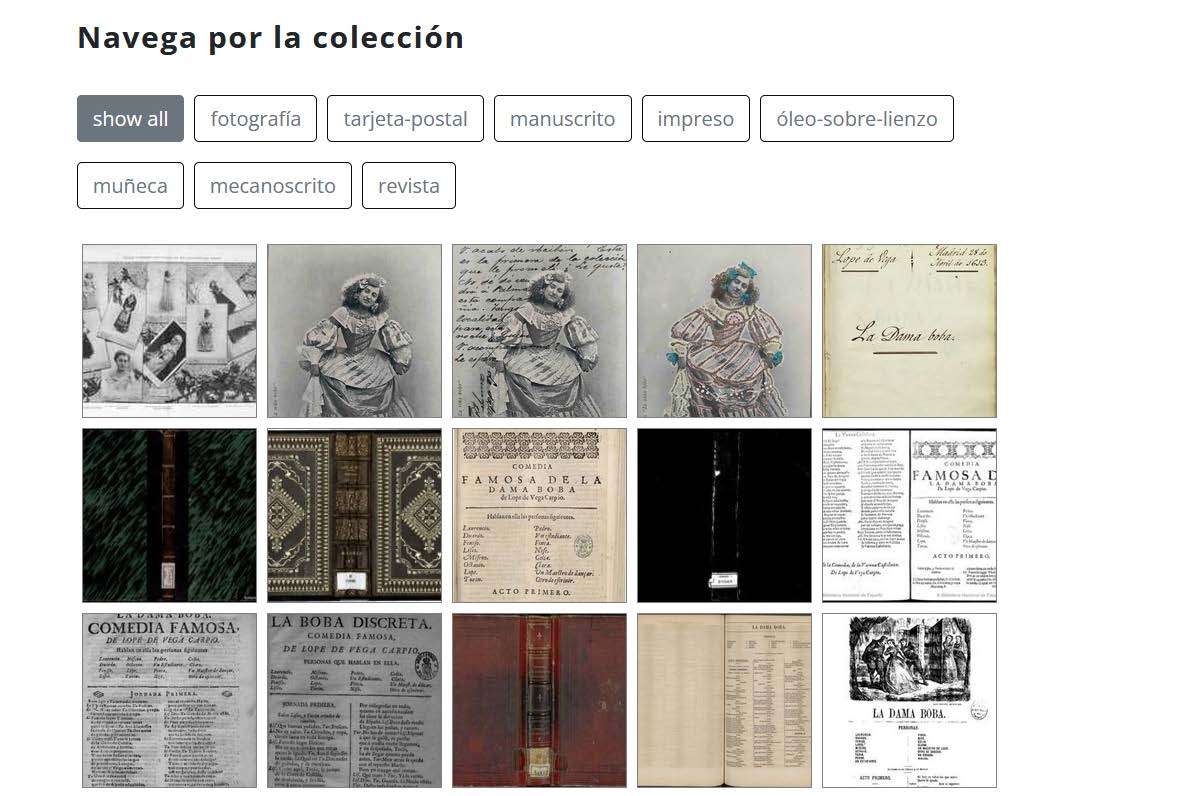
\includegraphics[keepaspectratio]{assets/mc-image5.jpg}}}

El proyecto \href{https://celioht.github.io/damaboba/}{\emph{La dama
boba: Archivo Crítico Digital}} emplea Minicomp/Wax para construir un
repositorio digital de objetos relacionados con la comedia de Lope de
Vega \emph{La dama boba}, abarcando desde textos críticos digitales
hasta pinturas, fotografías y otros materiales que han circulado a lo
largo del tiempo. Cada elemento incluye su origen y condiciones de
derechos, y cuando es posible, un enlace a su fuente original.

\href{https://hdlab.space/coleccion-foulche-delbosc/}{\pandocbounded{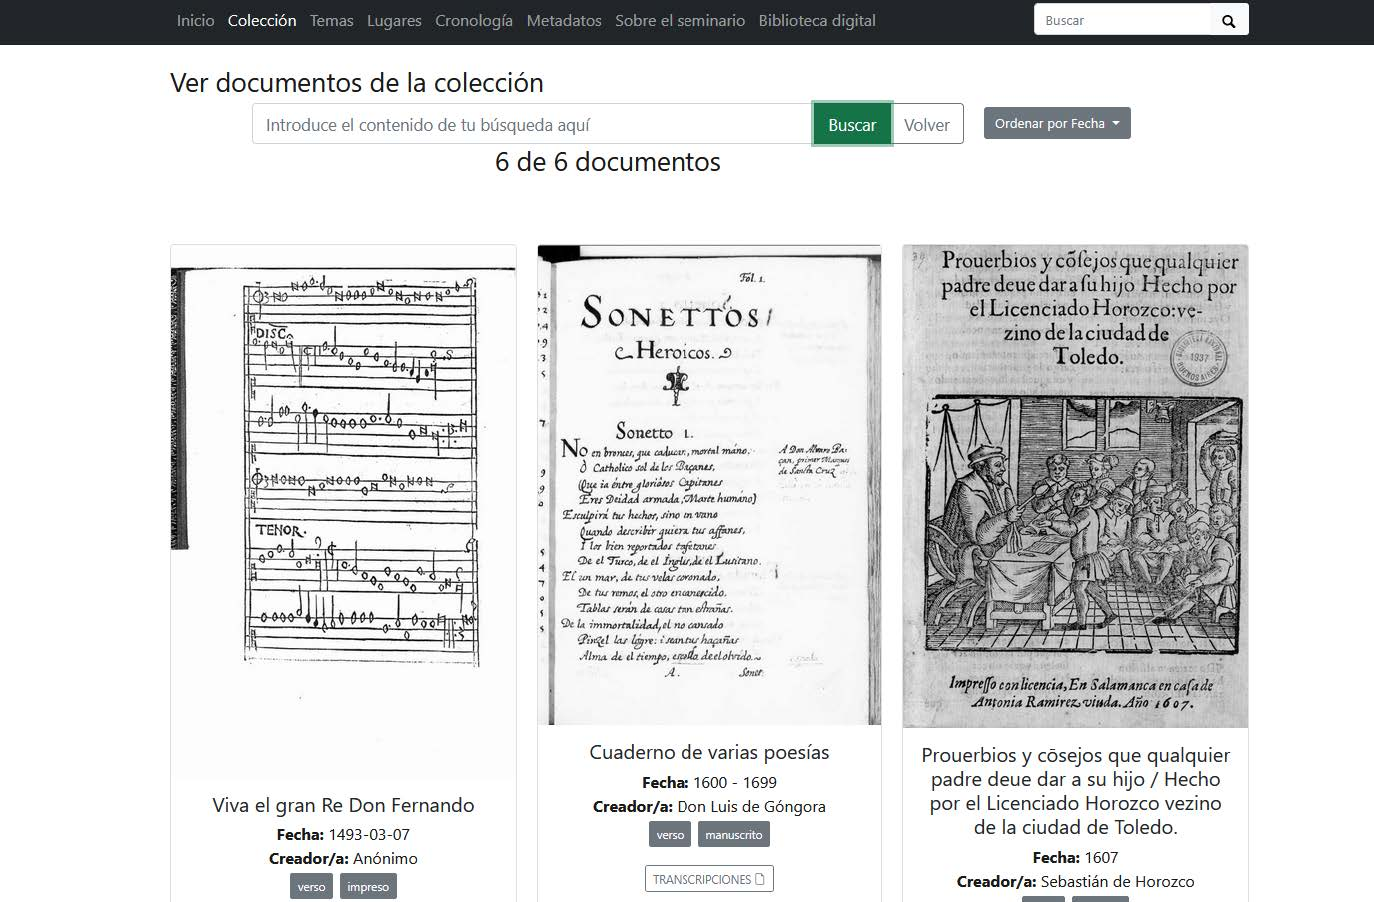
\includegraphics[keepaspectratio]{assets/mc-image6.jpg}}}

La \href{https://hdlab.space/coleccion-foulche-delbosc/}{Colección
Foulché-Delbosc} es una serie de ediciones diplomáticas digitales
desarrolladas por los participantes del seminario \emph{Historia del
Libro y la Edición a las Humanidades Digitales}, de la Facultad de
Filosofía y Letras de la Universidad de Buenos Aires (2024). El sitio
propone una exploración estructurada mediante filtros por cronología,
temas y lugares, además de brindar acceso directo a las transcripciones
codificadas en XML-TEI y a los metadatos en formatos abiertos como CSV y
JSON.

\section{Ética y sustentabilidad}\label{uxe9tica-y-sustentabilidad}

Las elecciones tecnológicas nunca son neutrales, ya que están mediadas
por condicionantes políticos, económicos y ambientales (Rio Riande,
2022a, p.~251). Desde esta perspectiva, optar por metodologías
vinculadas a la \emph{minimal computing} constituye también un gesto
crítico frente a los modelos de producción académica sostenidos
principalmente por instituciones del Norte Global. Al promover procesos
documentados, abiertos y reutilizables, este enfoque facilita la
transferencia de conocimientos y metodologías a contextos donde las
infraestructuras técnicas o el financiamiento son más limitados. De este
modo, no sólo se atenúan las brechas materiales en el acceso a recursos
tecnológicos, sino que también se fomenta la participación de
comunidades académicas más diversas en la producción del conocimiento
(Rio Riande, 2022b).

En el contexto latinoamericano, la adopción de la \emph{minimal
computing} ha tenido un impacto particular. La menor disponibilidad de
financiamiento y de infraestructuras técnicas en comparación con el
Norte Global ha convertido a esta metodología en una opción viable y, en
muchos casos, necesaria para garantizar la continuidad de proyectos de
investigación digital. Experiencias de creación de ediciones digitales,
repositorios de datos y plataformas de acceso abierto muestran cómo la
implementación de sitios estáticos y flujos de trabajo reproducibles ha
permitido sostener iniciativas con presupuestos limitados, al tiempo que
se forman comunidades académicas con mayor autonomía técnica. Tal como
señalan Viglianti et al.~(2022), esta perspectiva no solo facilita la
preservación de los proyectos, sino que también habilita prácticas
colaborativas y horizontales, donde estudiantes y jóvenes investigadores
encuentran espacios de participación a los que de otro modo no habrían
podido acceder.

La \emph{minimal computing} debe entenderse como una ética de la
investigación digital que articula sostenibilidad, autonomía y justicia
en la producción de conocimiento. Su relevancia para las Humanidades
Digitales radica tanto en su capacidad de reducir la dependencia de
infraestructuras complejas como en su potencial para democratizar el
acceso a metodologías y herramientas, especialmente en comunidades
académicas del Sur Global.

\bookmarksetup{startatroot}

\chapter{Contenido en Español}\label{contenido-en-espauxf1ol}

Uno de los mayores problemas para el desarrollo de un proyecto de
Humanidades es el de la sostenibilidad.

La historia de la informática en América Latina refleja los procesos de
modernización, dependencia tecnológica, y creatividad local en la
adopción y desarrollo de las tecnologías digitales.

\section{Primeras incursiones
(1950-1960)}\label{primeras-incursiones-1950-1960}

\textbf{Computadoras tempranas:} Las primeras computadores llegaron a
América Latina en los años 50, mayoritariamente importadas de Estados
Unidos o Europa. En general, fueron instalados en instituciones
gubernamentales, universidades o bancos.

\begin{itemize}
\item
  \textbf{Argentina:} La instalación de la Clementina en 1961 en el
  Instituto del Cálculo de la UBA (donada por la Universidad de
  Cambridge), bajo la dirección de Manuel Sadosky.\\
  \url{https://www.educ.ar/recursos/132323/pioneras-informaticas-rioplatenses}\strut \\
  \url{https://www.horaciocao.com.ar/wp-content/uploads/2015/05/08_Cuarenta_anos_de_informatica_en_el_Estado.pdf}
\item
  \textbf{Brasil:} Fundación del Centro de Procesamiento de Datos de la
  Universidad de São Paulo. IBM tuvo gran presencia.
\item
  \textbf{México:} Instalación de una UNIVAC en la UNAM en 1958.
\end{itemize}

\textbf{Educación y matemática aplicada:} Durante esta época se
desarrollaron programas formativos en matemáticas, estadística y cálculo
numérico, precursores de la computación científica.

\begin{center}\rule{0.5\linewidth}{0.5pt}\end{center}

\section{🏗️ Desarrollo incipiente y apropiación
(1970-1980)}\label{desarrollo-incipiente-y-apropiaciuxf3n-1970-1980}

\textbf{Surgimiento de la industria local:} Algunos países comenzaron a
fabricar computadoras o desarrollar software nacional.

\begin{itemize}
\tightlist
\item
  \textbf{Brasil:} Política de ``reserva de mercado'' que promovió la
  creación de empresas locales (Cobra Computadores).
\item
  \textbf{Cuba:} Desarrollo de sistemas propios como parte de su
  política de autosuficiencia tecnológica.
\item
  \textbf{Chile:} Proyecto Cybersyn (gobierno de Salvador Allende, con
  Stafford Beer), pionero en planificación económica asistida por
  computadoras.
\end{itemize}

\textbf{Educación universitaria:} Creación de carreras de computación e
informática en universidades públicas.

\begin{center}\rule{0.5\linewidth}{0.5pt}\end{center}

\section{💻 Globalización, neoliberalismo y expansión
(1990-2000)}\label{globalizaciuxf3n-neoliberalismo-y-expansiuxf3n-1990-2000}

\begin{itemize}
\tightlist
\item
  \textbf{Apertura de mercados:} Entrada masiva de tecnologías
  extranjeras (Microsoft, Oracle, IBM).
\item
  \textbf{Software libre:} Movimientos de adopción en el Cono Sur
  (Brasil, Venezuela).
\item
  \textbf{Brecha digital:} Mayor visibilidad de desigualdades
  urbano/rurales y sociales.
\end{itemize}

\begin{center}\rule{0.5\linewidth}{0.5pt}\end{center}

\section{🌐 Internet y digitalización
(2000-presente)}\label{internet-y-digitalizaciuxf3n-2000-presente}

\begin{itemize}
\tightlist
\item
  \textbf{Acceso masivo a Internet} y redes móviles.
\item
  \textbf{Políticas TIC:} Ej. Conectar Igualdad (Argentina), Plan Ceibal
  (Uruguay).
\item
  \textbf{Economía digital:} Startups en software, fintech, IA y
  biotecnología.
\end{itemize}

\begin{center}\rule{0.5\linewidth}{0.5pt}\end{center}

\section{🧠 Temas emergentes y desafíos
actuales}\label{temas-emergentes-y-desafuxedos-actuales}

\begin{itemize}
\tightlist
\item
  \textbf{Soberanía tecnológica}\\
\item
  \textbf{Educación e inclusión digital}\\
\item
  \textbf{Humanidades digitales y ciencia abierta} (ej. LA Referencia,
  RedHD, Asociación Argentina de Humanidades Digitales)
\end{itemize}

\begin{center}\rule{0.5\linewidth}{0.5pt}\end{center}

\section{🧭 ¿Qué es el software libre y por qué se
impulsó?}\label{quuxe9-es-el-software-libre-y-por-quuxe9-se-impulsuxf3}

El software libre permite usar, estudiar, modificar y distribuir
libremente el software. Ideal para:

\begin{itemize}
\tightlist
\item
  Reducir costos en gobiernos y universidades.
\item
  Evitar dependencia tecnológica.
\item
  Fomentar desarrollo local.
\item
  Favorecer transparencia pública.
\end{itemize}

\begin{center}\rule{0.5\linewidth}{0.5pt}\end{center}

\section{📌 Momentos clave y casos por
país}\label{momentos-clave-y-casos-por-pauxeds}

\subsection{🇧🇷 Brasil -- El caso más
emblemático}\label{brasil-el-caso-muxe1s-emblemuxe1tico}

2003-2010: Políticas nacionales de migración a software libre (ej.
Serpro).\\
Fórums Internacionales de Software Livre (FISL).

\subsection{🇻🇪 Venezuela -- Soberanía y ley de software
libre}\label{venezuela-soberanuxeda-y-ley-de-software-libre}

2004: Decreto 3.390 ordena migración del Estado.\\
Distribución Canaima Linux para educación.

\subsection{🇦🇷 Argentina -- Adopción
fragmentaria}\label{argentina-adopciuxf3n-fragmentaria}

Iniciativas en educación, municipios y agencias del Estado.\\
Ej.: Gleducar (2002), Conectar Igualdad (Huayra GNU/Linux).

\subsection{🇺🇾 Uruguay -- Plan Ceibal y código
abierto}\label{uruguay-plan-ceibal-y-cuxf3digo-abierto}

2007: Plan Ceibal con laptops y software libre.\\
2013: Ley de Software Libre en el Estado.

\subsection{🇨🇱 Chile -- Comunidad activa, menos respaldo
estatal}\label{chile-comunidad-activa-menos-respaldo-estatal}

Grupos como GNU Chile; migraciones parciales en ministerios y
municipios.

\begin{center}\rule{0.5\linewidth}{0.5pt}\end{center}

\section{📚 Bibliografía académica sobre software libre en América del
Sur}\label{bibliografuxeda-acaduxe9mica-sobre-software-libre-en-amuxe9rica-del-sur}

\begin{itemize}
\tightlist
\item
  Drahos, Peter; Braithwaite, John. \emph{Information Feudalism} --
  {[}ISBN 9781565848043{]}
\item
  Becker, Pablo; García, Julián (2014). \emph{Software libre, políticas
  públicas y Estado: apuntes sobre el caso argentino.}
  \url{https://rts.unq.edu.ar/article/view/203}
\item
  Almeida, Sérgio Amadeu da Silveira (2004). \emph{Software livre e
  inclusão digital.}
  \url{https://cienciaecultura.bvs.br/pdf/cic/v56n4/a13v56n4.pdf}
\item
  Peirano, Fernando (2009). \emph{Software libre en América Latina.}
  \url{https://repositorio.cepal.org/handle/11362/3776}
\item
  Marino, Marcela; Rubione, Florencia (2011). \emph{Educación y Software
  Libre: la experiencia de Gleducar.}
  \url{http://www.gleducar.org.ar/node/561}
\item
  Villanueva Núñez, Edgar David (2002). \emph{Carta abierta a
  Microsoft.}
  \url{https://www.gnu.org/philosophy/villanueva-response.es.html}
\item
  Saldías, Carlos; Astudillo, Javier (2007). \emph{Software libre en
  Chile: perspectivas y desafíos.}
\end{itemize}

\begin{center}\rule{0.5\linewidth}{0.5pt}\end{center}

\section{🌍 Epistemologías del Sur y pensamiento
decolonial}\label{epistemologuxedas-del-sur-y-pensamiento-decolonial}

\begin{itemize}
\tightlist
\item
  \textbf{Rita Segato:} \emph{La guerra contra las mujeres} (2016)\\
\item
  \textbf{María Lugones:} \emph{Hacia un feminismo descolonial} (2008)\\
\item
  \textbf{Lorena Cabnal:} Feminismo comunitario territorial\\
\item
  \textbf{Karina Bidaseca:} Epistemologías del sur, afrofeminismo
\end{itemize}

\textbf{Conceptos clave:} colonialidad del saber, locus de enunciación,
pensamiento fronterizo, epistemología insurgente, ecología de saberes.

\begin{center}\rule{0.5\linewidth}{0.5pt}\end{center}

\section{🌱 Saberes indígenas, campesinos y
afrodescendientes}\label{saberes-induxedgenas-campesinos-y-afrodescendientes}

Muchos pensadores y pensadoras desde movimientos sociales, territorios y
pueblos originarios han producido formas de conocimiento situado que no
siempre se inscriben en la academia.

\textbf{Ejemplos:}

\begin{itemize}
\tightlist
\item
  \textbf{Alicia Cawiya} (Ecuador, pueblo Achuar): defensora del
  conocimiento ancestral como base política y ecológica.
\item
  \textbf{Silvia Rivera Cusicanqui} (Bolivia): crítica decolonial del
  marxismo y la modernidad, con fuerte defensa del pensamiento
  \emph{ch'ixi} (dualidad no reconciliada).\\
  Ej.: \emph{Un mundo ch'ixi es posible} (2018).
\item
  \textbf{Frantz Fanon} (influencia desde el Caribe): aunque no
  latinoamericano, influyó en la conceptualización situada del
  conocimiento en contextos coloniales.
\end{itemize}

\begin{center}\rule{0.5\linewidth}{0.5pt}\end{center}

\section{📌 Principales conceptos}\label{principales-conceptos}

\begin{itemize}
\tightlist
\item
  \textbf{Colonialidad del saber} (Quijano)
\item
  \textbf{Locus de enunciación} (Mignolo)
\item
  \textbf{Pensamiento fronterizo}
\item
  \textbf{Epistemología insurgente / comunitaria / popular}
\item
  \textbf{Conocimiento encarnado y territorializado}
\item
  \textbf{Ecología de saberes} (Santos)
\item
  \textbf{Saberes no hegemónicos / subalternos}
\end{itemize}

\begin{center}\rule{0.5\linewidth}{0.5pt}\end{center}

\section{📅 Línea de tiempo -- Software libre en América del
Sur}\label{luxednea-de-tiempo-software-libre-en-amuxe9rica-del-sur}

\textbf{1990s}\\
💻 Chile, Argentina, Brasil: Surgen las primeras comunidades de usuarios
de GNU/Linux y grupos de software libre.\\
📚 Creación de LUGs (Linux User Groups) en universidades y foros
técnicos.

\textbf{2000-2004}\\
🇵🇪 2002: Proyecto de Ley en Perú sobre software libre en el Estado
(Villanueva vs.~Microsoft).\\
🇧🇷 2003: Gobierno de Lula promueve migración masiva a software libre en
agencias estatales.\\
🇻🇪 2004: Decreto 3.390 en Venezuela obliga al Estado a migrar a software
libre.\\
🇦🇷 2002: Nace Gleducar, proyecto educativo con software libre.

\textbf{2005-2010}\\
🇺🇾 2007: Plan Ceibal distribuye laptops con software libre en educación
primaria.\\
🇧🇷 Políticas nacionales de migración (Serpro, Caixa, Receita Federal).\\
🇻🇪 Desarrollo de Canaima GNU/Linux.\\
🇦🇷 Municipios (Morón, Rosario) adoptan software libre.\\
🌎 Expansión del Foro Internacional de Software Libre (FISL).

\textbf{2010-2015}\\
🇺🇾 2013: Ley de Software Libre en el Estado uruguayo.\\
🇦🇷 Se lanza Huayra GNU/Linux como sistema operativo educativo.\\
🇪🇨 Ecuador promueve el software libre en la administración pública.\\
🇻🇪 Canaima instalado en más de 2 millones de equipos.

\textbf{2015-presente}\\
🌐 Comunidad activa pero con menor impulso estatal.\\
🤖 Uso de software libre para IA, big data y educación.\\
👥 Vinculación con soberanía digital y datos abiertos.

\begin{center}\rule{0.5\linewidth}{0.5pt}\end{center}

\section{🧠 Reflexión final}\label{reflexiuxf3n-final}

La adopción del software libre en América del Sur fue un fenómeno tanto
tecnológico como político y cultural. En algunos países, como Brasil,
Venezuela o Uruguay, el Estado tuvo un rol central, mientras que en
otros el impulso vino de la sociedad civil y las comunidades técnicas.\\
En paralelo, los debates sobre \textbf{epistemologías del sur} y
\textbf{conocimiento situado} dialogan con la historia de la tecnología
en la región, subrayando la necesidad de \textbf{soberanía tecnológica},
\textbf{inclusión digital} y \textbf{reapropiación crítica de las
herramientas} para contextos locales.

See Knuth (1984) for additional discussion of literate programming.

\bookmarksetup{startatroot}

\chapter{English}\label{english}

Content in English.

\bookmarksetup{startatroot}

\chapter*{References}\label{references}
\addcontentsline{toc}{chapter}{References}

\markboth{References}{References}

\phantomsection\label{refs}
\begin{CSLReferences}{1}{0}
\bibitem[\citeproctext]{ref-knuth84}
Knuth, Donald E. 1984. {``Literate Programming.''} \emph{Comput. J.} 27
(2): 97--111. \url{https://doi.org/10.1093/comjnl/27.2.97}.

\end{CSLReferences}




\end{document}
